\section{Session and in-Session Experiments - Results} \label{sec:final-results}
From the results presented in previous sections of this chapter, we can then fix now the packet level variables for all the tests, since their effect has been studied in the previous sections of this chapter. The packet level configuration will be as follows:

\begin{itemize}
\item Packet Size distribution: A uniform packet distribution with an average of 768 bytes [512 - 1024 bytes] for all flows and for all sessions.
\item An exponential packet inter-arrival time distribution with some practical mean [e.g. 100 ms] for all flows and for all sessions.
\end{itemize}

\subsection{Session Number Experiment} \label{sec:gv_session_exp}
First of all we tested the session level. For this, we used the following parametrization for the session number, e.g. the number of \acs{WLAN} terminals in the \acs{AP} area:

\begin{itemize}
	\item Low session number: \textbf{3 sessions}.
	\item Medium session number: \textbf{9 sessions}.
	\item High session number: \textbf{18 sessions}.
\end{itemize}

\begin{figure}[h!]
	\centering
	\subfloat[3 sessions]{
		\label{fig:3sessions}
		\includegraphics[width=0.33\textwidth]{images/results/GlobalView/sessions/3sessions}
	}
	\subfloat[9 sessions]{
		\label{fig:9sessions}
		\includegraphics[width=0.33\textwidth]{images/results/GlobalView/sessions/9sessions}
	}
	\subfloat[18 sessions]{
		\label{fig:18sessions}
		\includegraphics[width=0.33\textwidth]{images/results/GlobalView/sessions/18sessions}
	}
	\caption{Session number experiment - User realizations}
	\label{fig:user_realizations_final}
\end{figure}

All the sessions were configured to arrive at the same time, at the beginning of the simulation, representing that the users had been in the network for a while and then the sensor starts estimating. In real terms, the sensors can be off while the \acs{WLAN} network is working in order to improve their energy efficiency. The sensors could be activated once some sessions are already in the network transmitting data. For this experiment, the number of flows per session and its inter-arrival times have been fixed in the way that was done before. The packet level has been randomized with the configuration presented at the beginning of this sub-section. We run a total of 25 runs with the same configuration for each one of the three cases. Figure \ref{fig:user_realizations_final} represents the user realizations for each one of the three load cases under study in this experiment.

First of all, we need to check if the mixture idle distribution can still be used for the different traffic configurations that are under test. Figure \ref{fig:sessions_composed_cdf} represents the \acs{CDF} of the idle function for the three load cases.

\begin{figure}[h!]
	\centering
	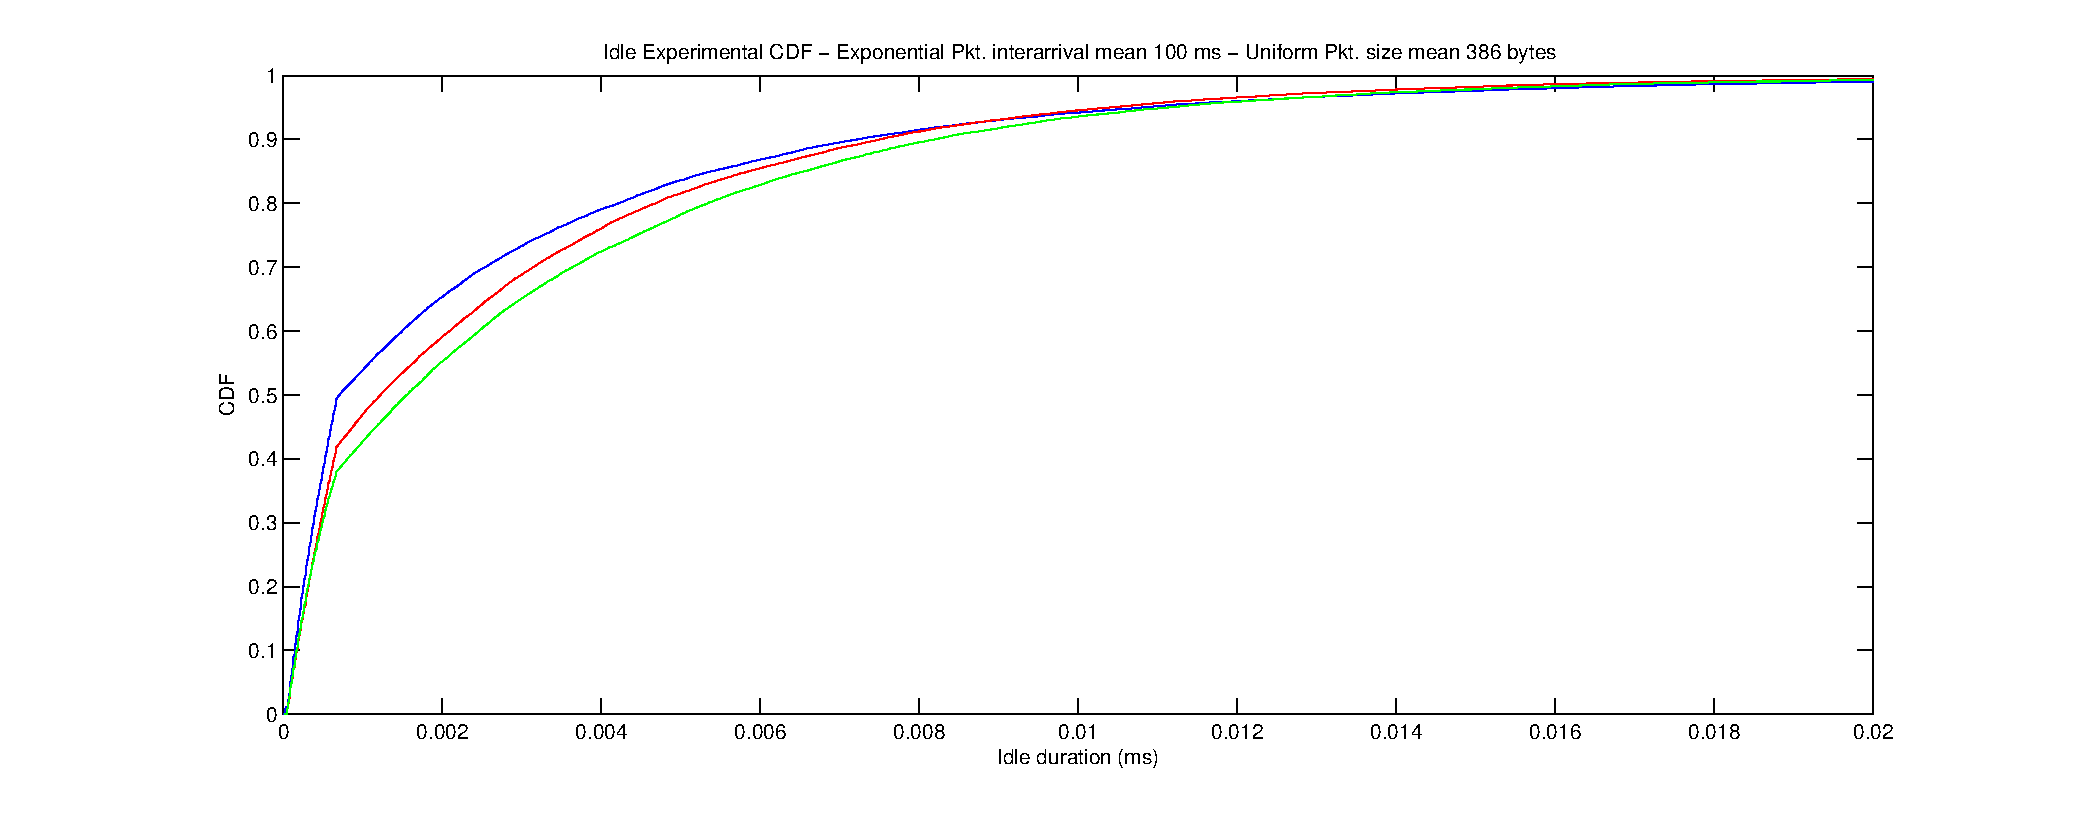
\includegraphics[width=1\textwidth]{images/results/GlobalView/sessions/sessions_composed_cdf}
	\caption{Idle distributions for different number of sessions}
	\label{fig:sessions_composed_cdf}
\end{figure}

As it can be observed in Figure \ref{fig:sessions_composed_cdf}, the mixture model can be used since two differentiated areas can be observed from the idle distributions: uniform distribution for $[0 < t < \alpha_{bk}]$ and a long-tail in $[t > \alpha_{bk}]$.

Since the mixture model can be applied in the three scenarios, it is necessary to check if the estimation process and validation test are being carried properly. For this, we extracted the estimated parameters and the \acs{K-S} values for the 25 runs of each case. It can be observed from Table \ref{table:session_test}, that the variability of the estimated parameters and the \acs{K-S} values can be considered negligible.

\begin{table}[h!]
	\centering
	\begin{tabular}{ c | c | c || c | c || c | c }
		& \multicolumn{2}{ c || }{3 sessions} &  \multicolumn{2}{ c || }{9 sessions} & \multicolumn{2}{ c }{18 sessions}\\ \hline \hline
		& Mean & Std. Dev. & Mean & Std. Dev. & Mean & Std. Dev. \\ \hline
		$\xi$ & 0.184869 & 0.0109214 & 0.0639 & 0.0095 & 0.025 & 0.0097 \\ 
		$\sigma$ & 0.00337252 & 4.80725e-05 & 0.0036 & 5.9426e-05 & 0.0045 & 6.27E-005 \\
		$p$ & 0.38928 & 0.00444004 & 0.2996 & 0.0057 & 0.2397 & 0.004 \\
		$p-value$ & 0.525856 & 0 0.253306 & 0.6874 & 0.2693 & 0.796 & 0.1874 \\ \hline
		$Fail$ & \multicolumn{2}{ c || }{0 \%} &  \multicolumn{2}{ c || }{0 \%} & \multicolumn{2}{ c }{0 \%}\\
	\end{tabular}
	\caption{Estimation parameters statistics for different number of sessions}
	\label{table:session_test}
\end{table}

The \acs{K-S} test shows also that there are no fails for the three session-cases under study, although, the results cannot be conclusive since are extracted from a 25-runs simulation. A higher numbers of runs are required to be statistically significant.

\subsection{In-session statistics} \label{subsec:globalview_insession}
The following experiment randomizes what is happening at the flow level. This level describes the behavior of individual sessions, e.g. \acs{WLAN} users. For this experiment we tested different number of sessions representing different load regions. Following the traffic model defined in \cite{Campus-WLAN}, and the results obtained in this chapter, the different levels of the multi-layer traffic model has been configured as it is presented in Table \ref{tab:sim_traffic_model}.

\begin{table}[h!]
	\begin{center}
		\begin{tabular}{ l | c | c }
			Modeled Variable & Distribution & Parameters \\ \hline
			Session number	& Fixed & N users arriving at simulator start \\
			Flow inter-arrival & Log-normal & $\mu = -1.6355$, $\sigma = 2.6286$ \\
			Flow number & Bi-Pareto & $\alpha = 0.07$, $\beta = 1.75$, $c = 295.38$, $k = 1$ \\
			Flow Size & Bi-Pareto & $\alpha = 0.00$, $\beta = 1.02$, $c = 15.56$, $k = 111$ \\
			Packet Size & Uniform & $min = 512$, $max = 1024$ \\
			Packet inter-arrival & Exponential & $\lambda = 10$ \\
		\end{tabular}
		\caption{The parameters used for generating traffic according to the model in \cite{Campus-WLAN}.}
		\label{tab:sim_traffic_model}
	\end{center}
\end{table}

The session cases under study in this these experiment are as follows:

\begin{itemize}
	\item 5 sessions - Standard traffic configuration.
	\item 5 sessions - Flow size magnified by 10.
	\item 10 sessions - Standard traffic configuration.
	\item 10 sessions - Flow size magnified by 10.
	\item 15 sessions - Standard traffic configuration. 
\end{itemize}

Session level (number of sessions and inter-arrivals) will be fixed for all the runs of each sub-experiment while the flow and packet levels will be randomized following the distributions presented in Table \ref{tab:sim_traffic_model}.



We studied two different load cases in this experiment. The configuration shown in Table \ref{tab:sim_traffic_model} with 5 sessions, give us a load range of 20\% - 45\%. In order to have a wider set of load cases, we magnified the flow-sizes by 10, which give a load range of 35\% - 65\%.

In Figure \ref{fig:limit_cdf_p} is represented the CDF of the P-value from the \acs{K-S} validation test. As it can be observed, for the lower load case, the failure rate is much lower than the one in the higher load case. In the high-load case, the network is saturated, which means that the number of samples gathered for the validation test is lower since we are validation the model over the truncated part ($sample > \alpha_{bk}$). In a higher load environment, the idle samples tend to be shorter and concentrated in the uniform part of the network. This behaviour is represented in Figure \ref{fig:limit_samples}. As it can be observed, the lower load case have a higher number of samples for the validation test since the idle samples are longer.

\begin{figure}[h]
	\centering
	\subfloat[]{
		\label{fig:limit_cdf_p}
		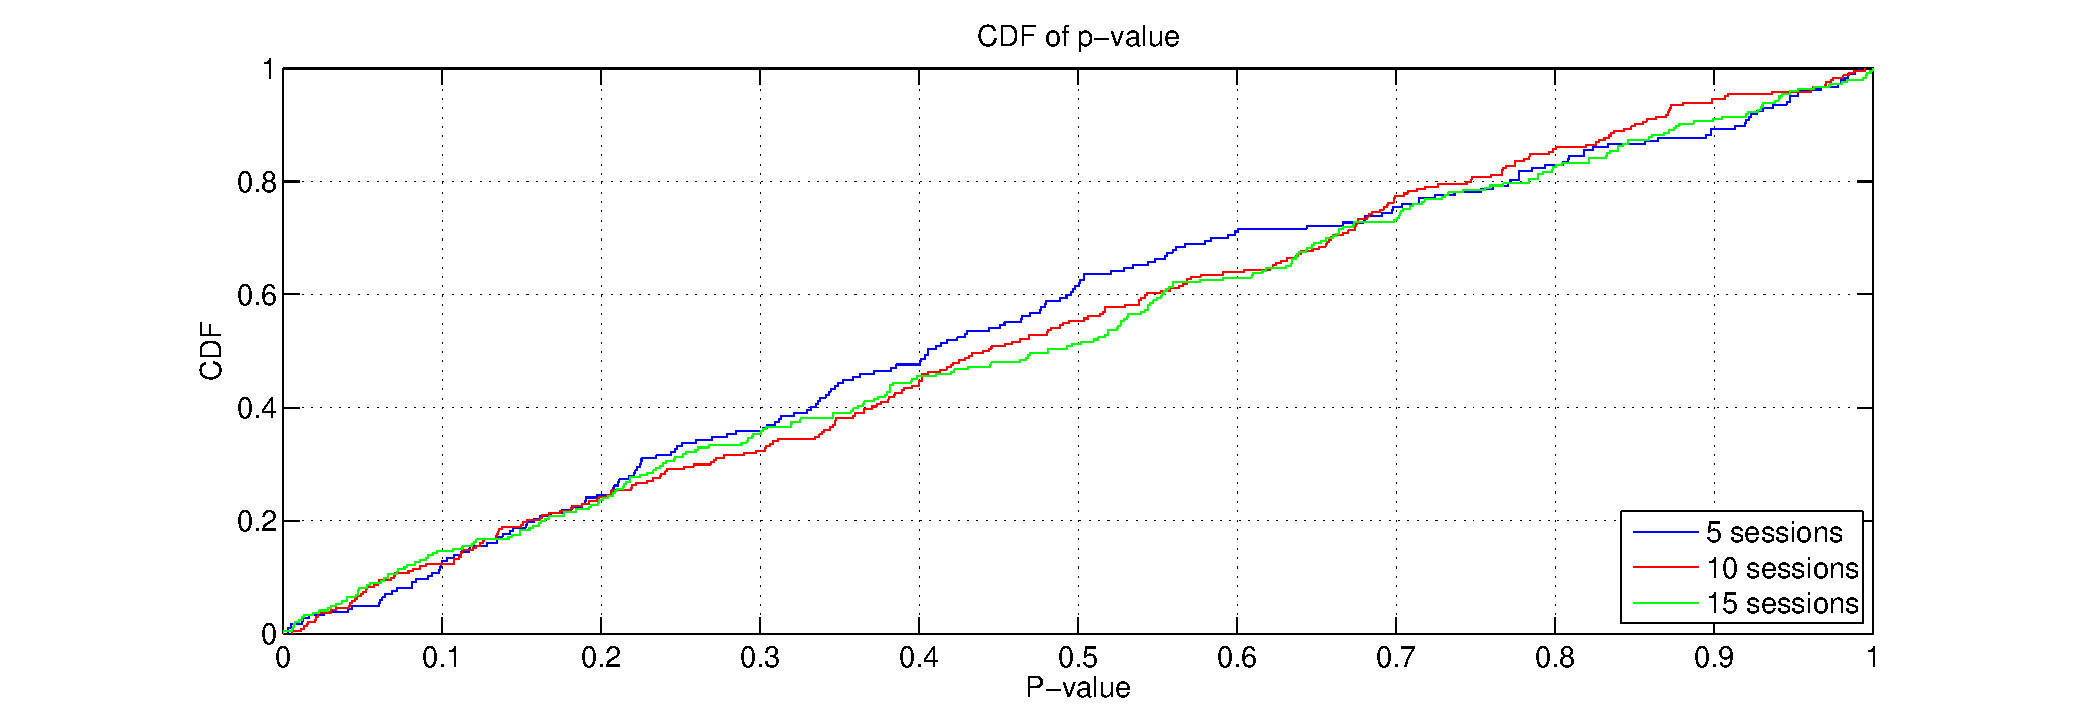
\includegraphics[width=0.5\textwidth, trim = 0mm 0mm 0mm 0mm, clip]{images/results/GlobalView/flows/limited_load/cdf_p}
	}
	\subfloat[]{
		\label{fig:limit_nflows}
		\includegraphics[width=0.5\textwidth, trim = 0mm 0mm 0mm 0mm, clip]{images/results/GlobalView/flows/limited_load/nflows}
	}
	\caption{CDF of p-value and flow number for reduced traffic model}
\end{figure}

\begin{figure}[h!]
	\centering
	\subfloat[]{
		\label{fig:limit_samples}
		\includegraphics[width=0.5\textwidth, trim = 0mm 0mm 0mm 0mm, clip]{images/results/GlobalView/flows/limited_load/samples}
	}
	\subfloat[]{
		\label{fig:limit_load}
		\includegraphics[width=0.5\textwidth, trim = 0mm 0mm 0mm 0mm, clip]{images/results/GlobalView/flows/limited_load/load}
	}
	\caption{CDF of number of valid samples and load in tests where $p-value<0.1$}
\end{figure}

We extracted also the load of those cases in which the \acs{K-S} failed. This is represented in Figure \ref{fig:limit_load}. As it can be observed, around 60\% of the cases, the load in the high-load case were above 46\% of load.

These figures show the results for all the cases in which the \acs{K-S} test failed. It is necessary to differentiate for different p-values. For this, we collected the data of the failed tests and divided in different regions using the p-value. From those results we obtained the mean value of the load and the number of valid samples. The results are presented in Table \ref{table:ks_fails_load_samples} and Figure \ref{fig:ks_fails_load_valid_samples_cdf}.

%\begin{table}[h]
%	\centering
%	\begin{tabular}{ l | c | c }
%		p-value & Load (\%) & Nr Valid Samples \\ \hline
%		0 to 0.02 & 38.16 & 12012 \\
%		0.02 to 0.04 & 33.57 & 15323 \\
%		0.04 to 0.06 & 31.69 & 15869 \\
%		0.06 to 0.08 & 32.23 & 14270 \\
%		0.08 to 0.1 & 34.13 & 14609 \\
%	\end{tabular}
%	\caption{Mean load and number of valid samples when $P<0.1$}
%	\label{table:ks_fails_load_samples}
%\end{table}

\begin{table}[h]
	\centering
    \begin{tabular}{c|c|c|c|c|c}
        Load region & \parbox{1.55cm}{5 sess. Std. Conf.} & \parbox{1.7cm}{5 sess. Magnified} & \parbox{1.6cm}{10 sess. Std. Conf.} & \parbox{1.7cm}{10 sess. Magnified} & \parbox{1.6cm}{15 sess. Std. Conf.} \\ \hline
        0 - 5 \%   & \textcolor{red}{0.0257}   & 0.121   & ~   & ~   & ~ \\ 
        5 - 10 \%  & 0.1543   & 0.1133    & \textcolor{red}{0.0188}   & \textcolor{red}{0.0105}   & \textcolor{red}{4.2263e-5}  \\ 
        10 - 15 \% & 0.4586   & 0.3922    & 0.1636    & \textcolor{red}{0.0665}   & \textcolor{red}{0.0570}  \\ 
        15 - 20 \% & 0.8338   & 0.6797    & 0.4954    & 0.2332                    & 0.3196                \\ 
        20 - 25 \% & 0.9616   & 0.8347    & 0.7959    & 0.5119                    & 0.6886                \\ 
        25 - 30 \% & 0.989    & 0.9339    & 0.9774    & 0.8210                    & 0.9240                \\ 
        30 - 35 \% & ~        & 0.9688    & ~         & 0.9514                    & 0.9899                \\ 
        35 - 40 \% & ~        & ~         & ~         & 0.9694                    & ~                     \\ 
        40 - 45 \% & ~        & ~         & ~         & 0.9771                    & ~                     \\ 
        45 - 50 \% & ~        & ~         & 0.9951    & 0.9915                    & ~                     \\ 
        50 - 55 \% & 0.9911   & ~         & ~         & 0.9962                    & ~                     \\ 
        55 - 60 \% & ~        & ~         & ~         & ~                         & 0.9985                \\ 
        60 - 65 \% & ~        & ~         & ~         & ~                         & 0.9998                \\
    \end{tabular}
	\caption{Load regions and related p-value from KS test}
	\label{table:load_regions}
\end{table}

\begin{figure}[h!]
	\centering
	\includegraphics[scale=0.5, trim = 0mm 0mm 0mm 0mm, clip]{images/results/GlobalView/flows/limited_load/cdf_of_valid}
	\caption{CDF of number of valid samples for different ranges in p-value}
	\label{fig:ks_fails_load_valid_samples_cdf}
\end{figure}

\textcolor{red}{ It can be observed that for each region of p-value, the mean load and the mean number of valid samples is different. When the p-value is really low, the load is quite higher than the case in which the p-value is around the considered null-hypothesis frontier. Also, the number of valid samples is almost the half as the other cases.}

\textcolor{red}{ The different results obtained in these set of experiments make us to reconsider the proposed model. The results obtained show that for high loads the estimation failed. On the other hand, the results also show that most of the cases in which the validation test failed for a lower load, the load is higher than 60\% and the number of valid samples is around 25\% of the gathered samples. In order to obtain enough valid samples in cases with moderate-high load the sensor needs to be active for a longer time since most of the samples are in the saturated region of the network affecting the energy-efficiency of the system. As a future work, one possible approach to modify the model is to avoid the estimation process for those high-load cases improving the energy-efficiency of the sensors.}